% !TeX root = ../Notizen.tex
\section*{Aufgabe 2: Poincaré Schnitt}
Bei niedrigen Fällen wie in Aufgabe 1 liegt eine Harmonische Schwingung vor.
Wenn die Energie größer wird tritt chaotisches Verhalten auf.
Bei noch größeren Energien kehrt das System in ein quasi periodischen Zustand zurück.
Anfangsbedingung für die Beiden Fälle sind hier aufgelistet.
\begin{align}
	\theta_{1,\text{chaos}}=&0,0 \hspace{50pt} \dot{\theta}_{1,\text{chaos}}=0,0\nonumber\\
	\theta_{2,\text{chaos}}=&0,0 \hspace{50pt} \dot{\theta}_{2,\text{chaos}}=4,472\hspace{50pt}E=E_\text{kin}=\SI{10}{\joule}\\
	\theta_{1,\text{quasi}}=&0,0 \hspace{50pt} \dot{\theta}_{1,\text{quasi}}=0,0\nonumber\\
	\theta_{2,\text{quasi}}=&0,0 \hspace{50pt} \dot{\theta}_{2,\text{quasi}}=11,832\hspace{50pt}E=E_\text{kin}=\SI{70}{\joule}
\end{align}
\subsection*{a)}
Die Phasenraumbilder für die drei betrachteten Fälle sind in \cref{fig:phasenraum1,fig:phasenraum2,fig:phasenraum3} dargestellt.
\begin{figure}[h!]
	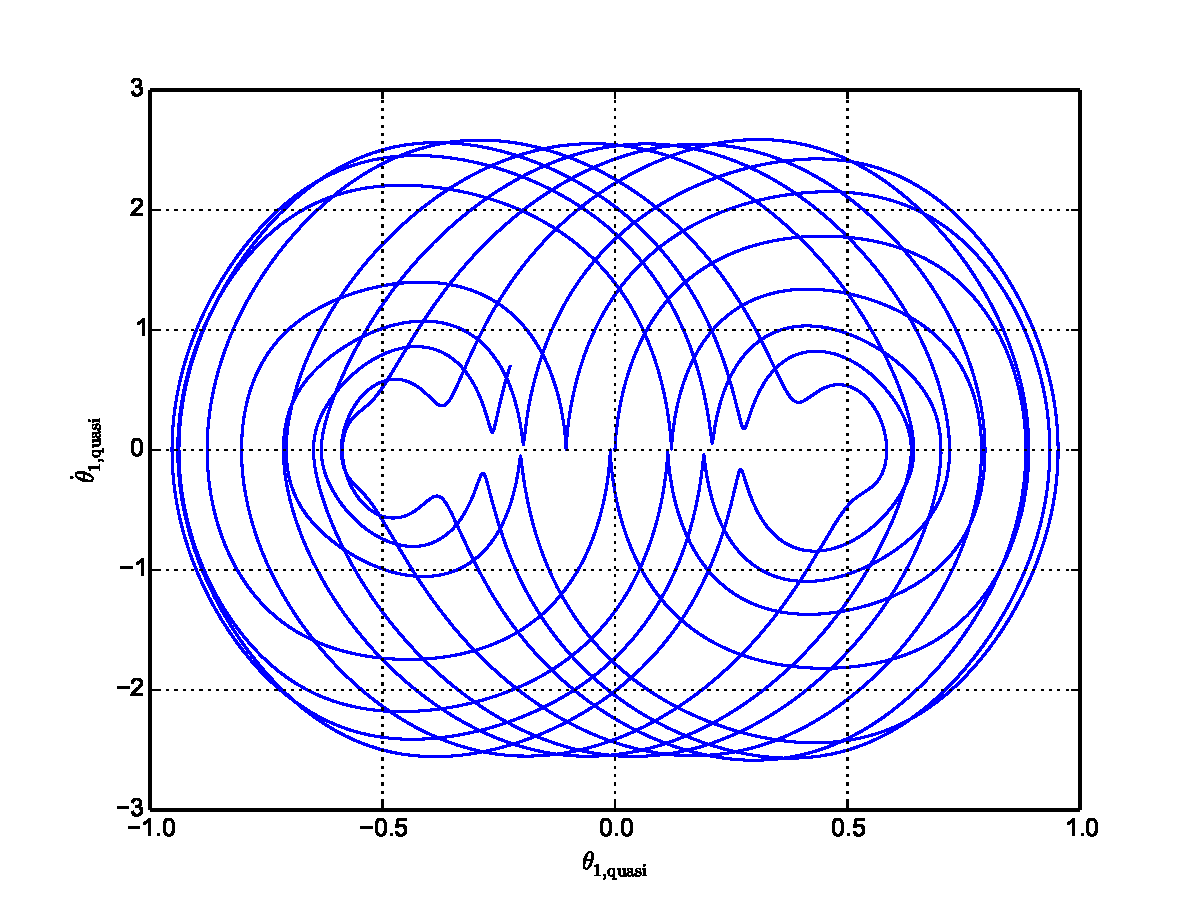
\includegraphics[width = \textwidth]{../Plots/Plot_2_A_1_Phasenraum.pdf}
	\caption{Phasenraum für quasiperiodisches Verhalten.\label{fig:phasenraum1}}
\end{figure}

\begin{figure}[H]
	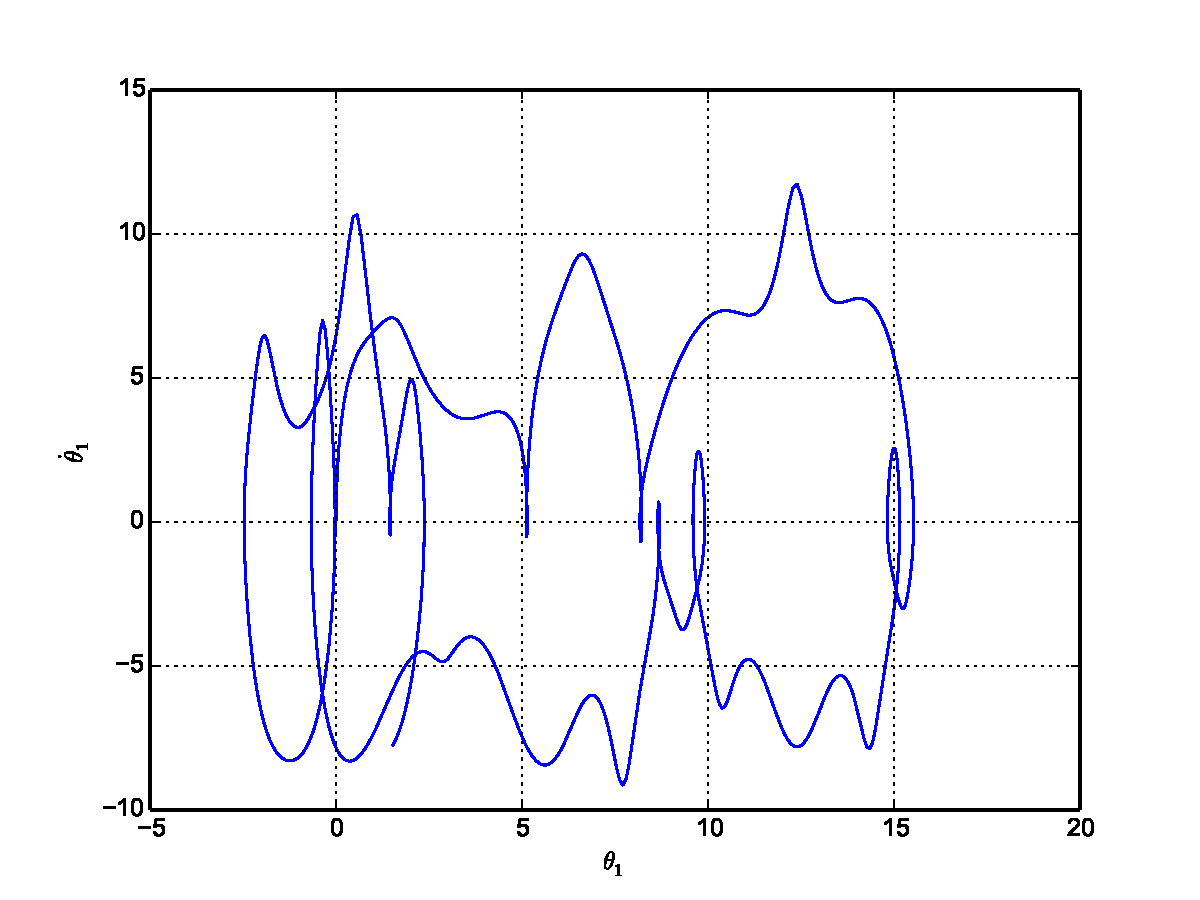
\includegraphics[width = \textwidth]{../Plots/Plot_2_A_2_Phasenraum.pdf}
	\caption{Phasenraum für chaotisches Verhalten.\label{fig:phasenraum2}}
\end{figure}

\begin{figure}[H]
	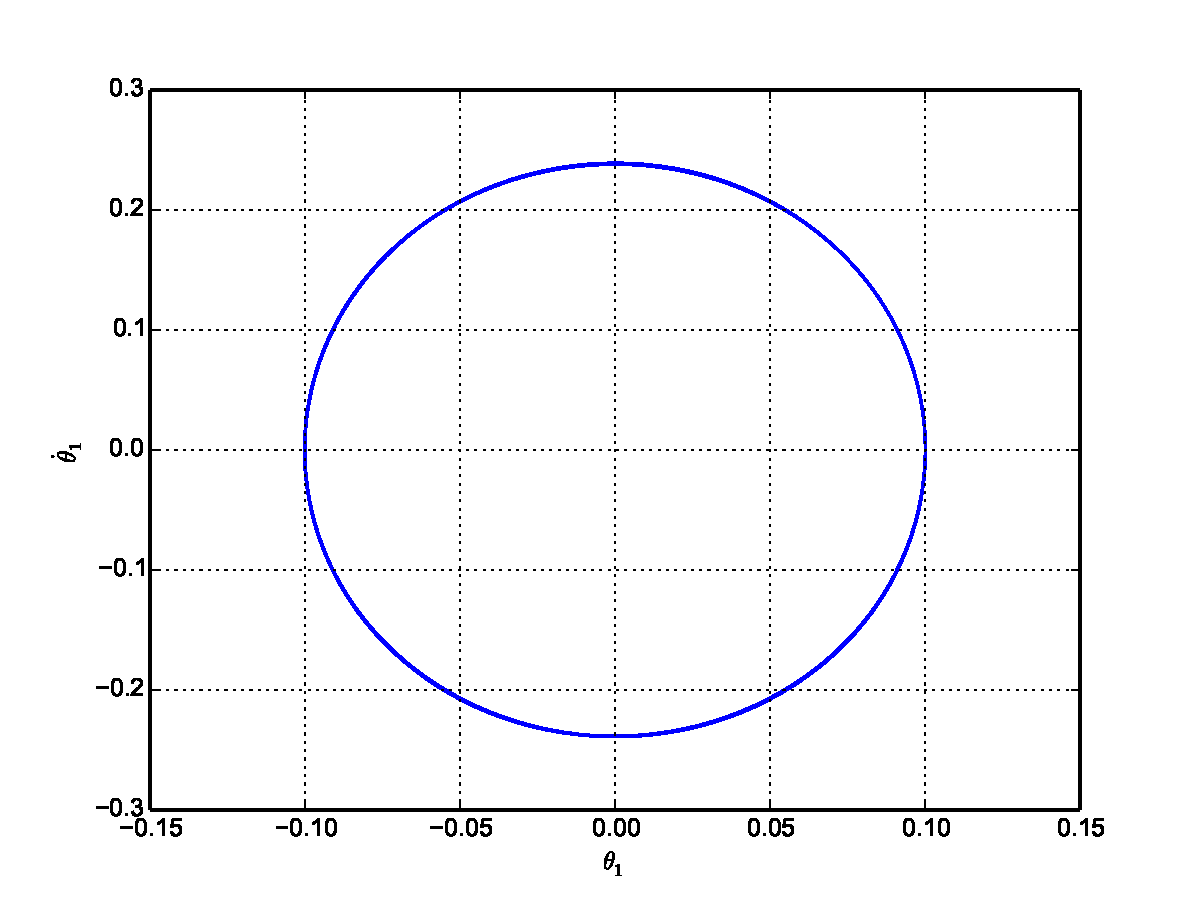
\includegraphics[width = \textwidth]{../Plots/Plot_2_A_3_Phasenraum.pdf}
	\caption{Phasenraum für periodisches Verhalten ($\theta_2=\sqrt{2}\theta_1$).\label{fig:phasenraum3}}
\end{figure}

\newpage\newpage
\subsection*{b)}
Der Abstand der quasiperiodischen Schwingung von der ungestörten ist in \cref{fig:abstand1} dargestellt.
\begin{figure}[H]
	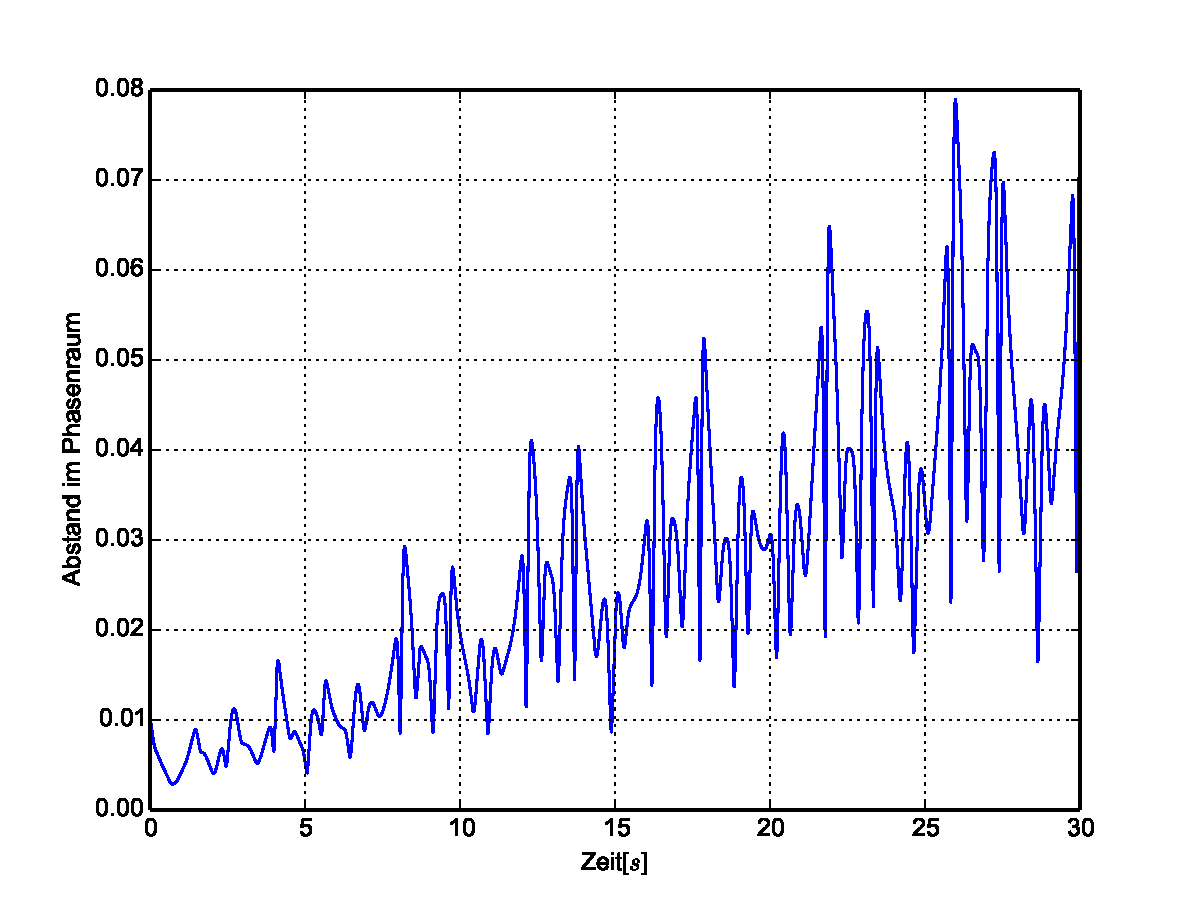
\includegraphics[width = \textwidth]{../Plots/Plot_2_B_1.pdf}
	\caption{Abstand der Trajektorie der quasiperiodischen Schwingung von der ungestörten in Abhängigkeit von der Zeit $t$.\label{fig:abstand1}}
\end{figure}
Der Abstand der chaotischen Dynamik von der ungestörten Schwingung ist in \cref{fig:abstand2} dargestellt.
\begin{figure}[H]
	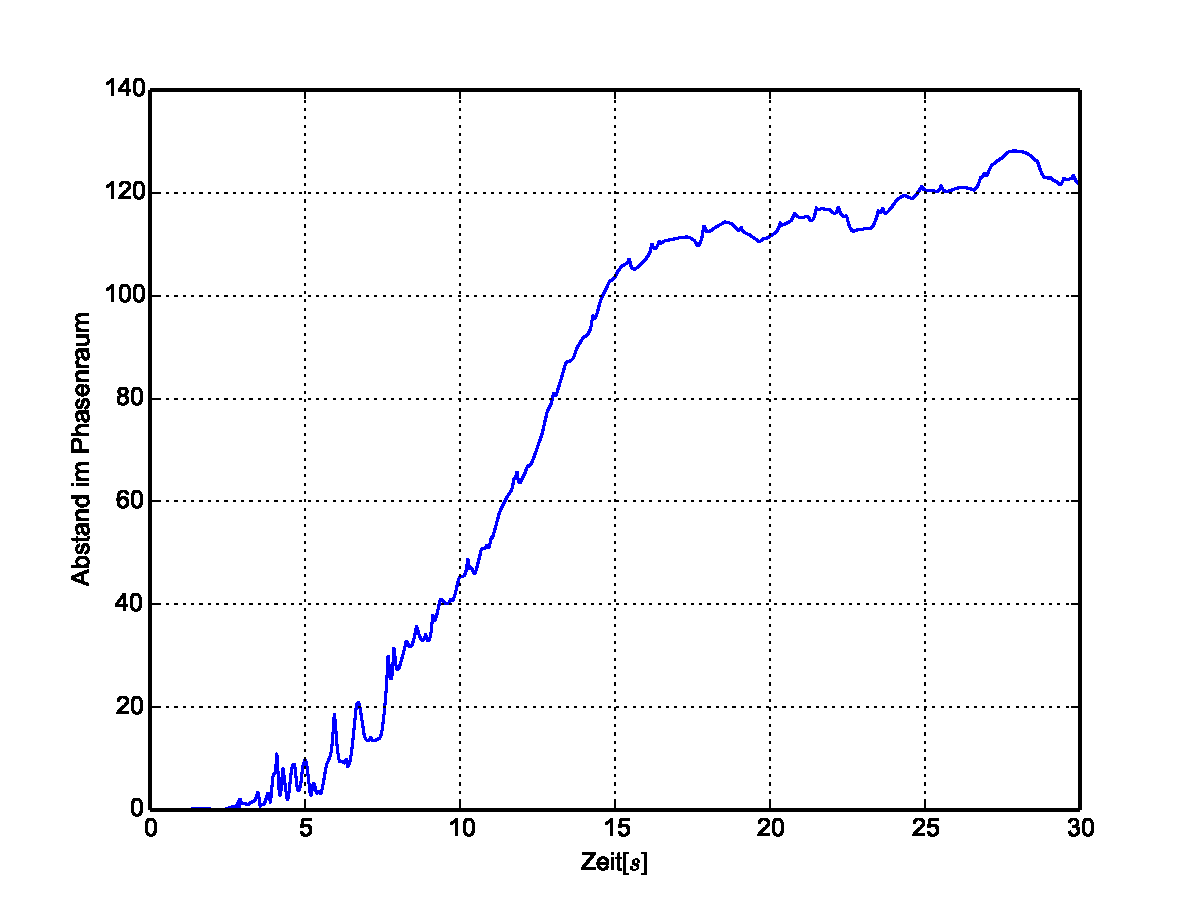
\includegraphics[width = \textwidth]{../Plots/Plot_2_B_2.pdf}
	\caption{Abstand der Trajektorie mit chaotischer Dynamik von derjenigen der ungestörten Schwingung in Abhängigkeit von der Zeit $t$.\label{fig:abstand2}}
\end{figure}

\subsection*{c)}
Es werden die Poincaré Schnitte berechnet.
Dabei werden werte gewählt bei denen $\theta_2=0$ und es gilt $\dot{\theta_2}+\lambda\dot{\theta_1}\cos\theta_1>0$ gilt.
Hier für werden verschiedene Anfangsbedingungen mit gleicher Energie berechnet.
\begin{align}
	E&=E'\\
	\frac{1}{2}\dot{\theta}_2^2&=\frac{g}{\SI{1}{\meter}}(3-2\cos(\theta_1')-\cos(\theta_2')) + \frac{1}{2}\left( 2\dot{\theta}'_1^2 +\dot{\theta}'_2^2 + 2\cos(\theta_1'-\theta_2')\dot{\theta}'_1\dot{\theta}'_2 \right)
\end{align}
Mithilfe dieser Gleichung lassen sich nun verschiedene Startbedingungen bestimmen.
Es müssen nur Relationen zwischen den gestrichen Koordinaten gemacht werden.
Zum Beispiel
\begin{align}
	\theta_1'=\tehta_2' =0=\dot{\theta}_2'\\
	\Rightarrow \dot{\theta}_2'=\frac{1}{\sqrt{2}}\dot{\theta}_2.
\end{align}